\section{Experiments}
\label{sec:experiments}

The experiments answer five questions. \textbf{RQ1}: do logged rollouts support the two-channel model of \Cref{sec:two_channel}, and do the measured constants reproduce the predictions of \Cref{sec:cis}? \textbf{RQ2}: inside one RL system and under one recipe, does the deployed operator improve held-out accuracy and training stability over the cap, the gate, and the exact ratio? \textbf{RQ3}: which elements of the operator matter, and in which direction? \textbf{RQ4}: can the slope be compiled from measurements, and does the compiled slope transfer across serving configurations as the proportionality $\lambda_+=c\tau^\star$ of \Cref{thm:cis_informal} prescribes? \textbf{RQ5}: which tokens does the band act on during training? Section~\ref{sec:experiments-setup} describes the shared setup; each subsequent subsection answers one question. Implementation details and additional tables and figures are in Appendix~\ref{app:experimental}.

\subsection{Setup}
\label{sec:experiments-setup}

\noindent\textbf{Mismatch measurement.}\label{sec:exp_measurement}
We measure $(k_t,p_t)$ on 12.3M tokens of Qwen1.5-MoE-A2.7B-Chat and 12.4M tokens of a dense control (Qwen1.5-14B-Chat): vLLM samples eight responses per DAPO-Math prompt at temperature one and records each sampled token's log-probability at the sampling step, and the training engine rescores the same sequences at the same parameters. Controls, the paired stale-snapshot measurement behind Figure~\ref{fig:two_channel}, and training-time logging are in Appendix~\ref{app:experimental-diagnostics}.

\noindent\textbf{Training.}
We train Qwen1.5-MoE-A2.7B-Chat with AReaL on the GSM8K training set (SGLang rollouts, FSDP training, both bf16) and report greedy exact-match accuracy on the 1{,}319 held-out test problems (standard error about $1.3$ points per arm), with three seeds per method and one further run per method with the KV cache quantized to FP8. All arms share one recipe and code path (Appendix~\ref{app:experimental-implementation}) and differ only in the operator: no correction, the exact ratio, TIS (cap $2$), IcePop (mask $[0.5,5]$), the binary-KL mask of AReaL (KPop, threshold $2$), and CIS (\Cref{alg:cis}, $\lambda_+=2.3$, $\kappa=5\times10^{-3}$).

\subsection{RQ1: Do rollout logs support the two-channel model?}
\label{sec:experiments-diagnostics}

\begin{figure}[t]
\centering
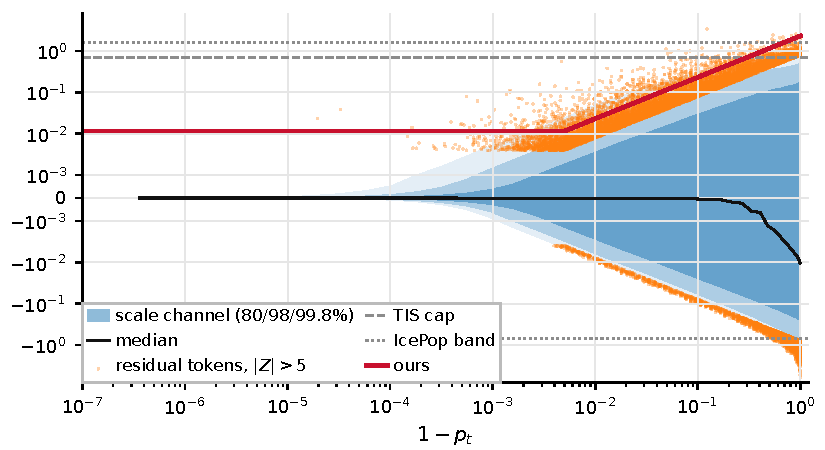
\includegraphics[width=\linewidth]{figures/mechanism.pdf}
\caption{Conditional distribution of $\log k_t$ against training-side uncertainty $1-p_t$ on the MoE model (12.3M tokens; symmetric-log vertical axis). Blue bands are the central 80\%, 98\%, and 99.8\% of tokens per uncertainty bin and follow the scale family of \Cref{def:two_channel} over six decades; the black line is the conditional median. Orange points are residual tokens with $|Z_t|>5$; at high confidence they lie above the shrinking bulk and are almost all positive. Grey lines are the constant thresholds of TIS ($\log 2$, dashed) and IcePop ($\log 0.5$ and $\log 5$, dotted), which lie above the entire distribution except at the least confident tokens. The red curve is the deployed one-sided band of \Cref{alg:cis}; its floor $\lambda_+\kappa=0.0115$ meets the residual layer at high confidence.}
\label{fig:mechanism}
\end{figure}

\noindent\textbf{Scale channel.}
Throughout this section $\varphi_t:=\max(1-p_t,\kappa)$ denotes the floored uncertainty of \Cref{alg:cis}, and $Z_t:=\log k_t/(c\varphi_t)$ the standardized deviation. Figure~\ref{fig:mechanism} shows the conditional distribution of $\log k_t$. Its width follows the scale family of \Cref{def:two_channel} across six decades of uncertainty, with $c=0.155$ for the MoE model and $c=0.035$ for the dense model and a weighted $R^2$ of $0.998$ over twenty equal-mass bins. After standardization by $c\varphi_t$ the central quantiles of $Z_t$ collapse across bins: between $\varphi=5\times10^{-3}$ and $\varphi=1$ the median moves by $0.06$ and the two deciles by $0.35$ and $1.17$ (Figure~\ref{fig:pivot}a). The upper tail is generalized Pareto with $\xi_+=0.49$ above the 99th percentile for the MoE model and $\xi_+=0.07$ for the dense model, so the MoE tail is heavy and some truncation is necessary rather than optional.

\noindent\textbf{Residual channel.}
We call a token residual when $|Z_t|>\zeta$ with the preregistered $\zeta=5$. Residual tokens are sparse, with $\hat\epsilon=1.26\%$ ($2.16\%$ at $\zeta=4$ and $0.78\%$ at $\zeta=6$), and their indicator is uncorrelated with $\varphi_t$ (correlation $0.004$). They cluster only weakly within trajectories: the lag-one autocorrelation of the indicator is $0.041$ against a permutation null of $0.0002$, and the conditional lift decays from $4.2$ at lag one to $2.6$ at lag four. At high confidence ($\varphi<0.05$) the residual displacement is one-sided, with $97.7\%$ of residual tokens positive on the base model and $100\%$ on the trained policy, and it is bounded, with a 99th percentile of $0.33$. Residual tokens are enriched in hard routing flips, which we define as a route change with gate margin above $10^{-3}$, by a factor of $1.46$ over the base rate of $0.53$, and they carry $2.0$ flipped layers on average against $1.1$ overall; the enrichment is real but not decisive, so routing is one contributor to the residual channel rather than its only cause. On the base model the residual median magnitude still scales with $\varphi$, at a fixed factor of about six above the bulk (Figure~\ref{fig:dualscale}a). The non-scaling behavior of \Cref{def:two_channel} appears once the policy has been trained and once the two engines are displaced in version. On the same tokens scored under a snapshot that is 29 steps stale, and in the logs of the training run itself, the residual magnitude at $\varphi<0.02$ lies between $0.04$ and $0.11$ while $c\varphi$ lies one to two orders of magnitude below it (Figure~\ref{fig:dualscale}b,c). We therefore state the non-scaling envelope as a high-confidence property, which is the regime in which \Cref{thm:cis_informal} is invoked. The paired measurement also fixes the sign structure of version displacement: rescoring the same tokens under the same snapshot through the two decode paths gives exactly zero difference, the displacement between snapshots is two-sided overall ($48.9\%$ positive) with a negative median at low confidence which reflects policy sharpening, and it is entirely positive on the high-confidence residual tokens that the operator acts on.

\noindent\textbf{Null measurements on the $\epsilon=0$ section.}
When $\epsilon=0$ the robust risk~\eqref{eq:robust_risk} reduces to an average-case criterion, and such criteria do not produce a confidence-dependent band; the band is a consequence of $\epsilon>0$. Four independent measurements on the same logs agree with this prediction. The sequence-level surface $\Delta(\varphi)$ has slope $-0.002$ with a trajectory-bootstrap interval of $[-0.48,0.15]$ over $20{,}000$ trajectories; the coupling coefficient $\lambda_{\mathrm{eff}}=c(\beta_1-\tfrac32\beta_2)$ has an interval which covers zero in three independent batches; the bare leave-one-out sum has slope $0.31$ against $\varphi$, of which $0.25$ survives a permutation that destroys within-trajectory coupling; and best-response iteration of the sequence-level risk converges from every start to a constant cap with $\lambda^\star=0.07$. The cross-layer coherence check gives a far-layer gradient coherence of $0.10$ between confidence layers, which is indistinguishable from its permutation null, and within a layer the token gradient directions are nearly orthogonal ($\rho\approx0.005$). RQ1 is therefore answered in the affirmative for the scale channel and for the sparsity, sign, and boundedness of the residual channel, with the qualification that the non-scaling envelope is a high-confidence property.

\subsection{RQ2: Does the operator improve accuracy and stability over the cap and the gate?}
\label{sec:experiments-results}

\begin{table}[t]
\centering
\caption{Held-out GSM8K accuracy (\%) after three epochs with three seeds per method, same recipe and code path for all methods; the untrained model scores $52.31$. Training reward is the mean over the third epoch, and intervened tokens is the fraction of loss tokens that the operator truncated or masked, both for seed one and as reported by the training framework. All methods take $31$ to $34$ seconds per optimizer step on the same hardware; no operator adds a forward or backward pass. The three leading methods lie within one standard error of one another; the deployed operator has the highest mean, the smallest spread, and the highest worst seed.}
\label{tab:main}
\small\setlength{\tabcolsep}{4pt}
\begin{tabular}{lcccccc}
\toprule
Method & Seed 1 & Seed 2 & Seed 3 & Mean $\pm$ std & Train reward & Intervened (\%) \\
\midrule
No correction ($M\equiv1$) & 56.10 & 54.44 & 56.10 & $55.55\pm0.96$ & 0.73 & 0 \\
Exact ratio ($M=k$) & 64.59 & 55.50 & 59.06 & $59.72\pm4.58$ & 0.843 & 0 \\
KPop (binary-KL mask, $2$) & 59.44 & 59.29 & 57.85 & $58.86\pm0.88$ & 0.852 & 21.9 \\
IcePop (mask $[0.5,5]$) & \textbf{64.82} & 62.70 & 63.46 & $63.66\pm1.07$ & 0.855 & 4.1 \\
TIS (cap $2$) & 62.40 & 63.91 & \textbf{65.43} & $63.91\pm1.52$ & 0.847 & 0.8 \\
CIS (ours, \Cref{alg:cis}) & 64.67 & \textbf{64.97} & 63.23 & $\mathbf{64.29\pm0.93}$ & \textbf{0.867} & 4.2 \\
\bottomrule
\end{tabular}
\end{table}

\begin{figure}[t]
\centering

\includegraphics[width=0.9\linewidth]{figures/dyn_legend.pdf}\\[2pt]
\begin{minipage}[t]{0.325\linewidth}\centering
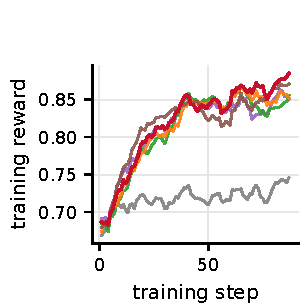
\includegraphics[width=\linewidth]{figures/dyn_reward.pdf}\\[-2pt]{\small (a)}
\end{minipage}\hfill
\begin{minipage}[t]{0.325\linewidth}\centering
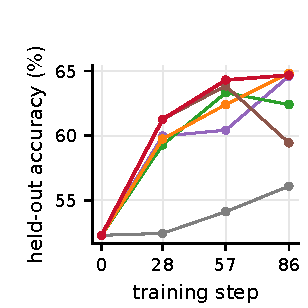
\includegraphics[width=\linewidth]{figures/dyn_heldout.pdf}\\[-2pt]{\small (b)}
\end{minipage}\hfill
\begin{minipage}[t]{0.325\linewidth}\centering
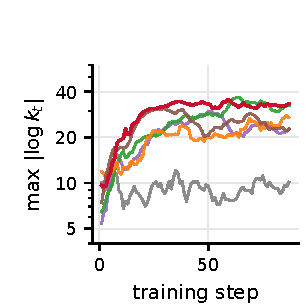
\includegraphics[width=\linewidth]{figures/dyn_gapmax.pdf}\\[-2pt]{\small (c)}
\end{minipage}\\[4pt]
\begin{minipage}[t]{0.325\linewidth}\centering
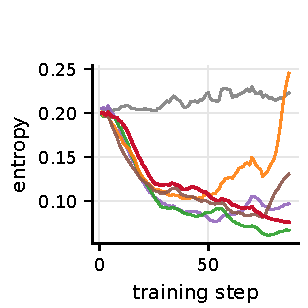
\includegraphics[width=\linewidth]{figures/dyn_entropy.pdf}\\[-2pt]{\small (d)}
\end{minipage}\hfill
\begin{minipage}[t]{0.325\linewidth}\centering
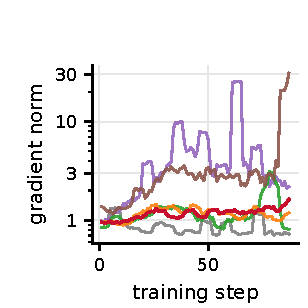
\includegraphics[width=\linewidth]{figures/dyn_grad.pdf}\\[-2pt]{\small (e)}
\end{minipage}\hfill
\begin{minipage}[t]{0.325\linewidth}\centering
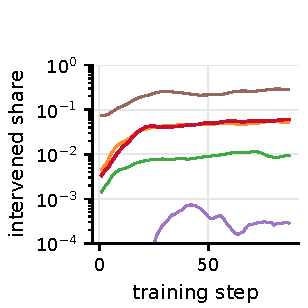
\includegraphics[width=\linewidth]{figures/dyn_rs.pdf}\\[-2pt]{\small (f)}
\end{minipage}
\caption{Training dynamics of the six operators under one recipe (seed one; curves smoothed over five steps). (a) Training reward. (b) Held-out accuracy of the epoch checkpoints, starting from the untrained model: the deployed operator leads at every checkpoint ($61.3$, $64.3$, $64.7$), and the KL mask peaks at $63.8$ after two epochs and falls to $59.4$ in the last one. (c) Largest $|\log k_t|$ in the batch, which grows during training for every corrected run as the policy sharpens. (d) Policy entropy. (e) Gradient norm: the exact ratio is spiky and the KL mask diverges late, whereas the cap, the gate, and the band stay near one. (f) Fraction of loss tokens intervened on by each operator; the KL mask removes about a fifth of all tokens.}
\label{fig:dynamics}
\end{figure}

Table~\ref{tab:main} reports held-out accuracy for six operators applied to the same pair $(k_t,p_t)$ in the same code, and Figure~\ref{fig:dynamics} shows their training dynamics. Correcting the mismatch in any bounded way adds $8.7$ points over the uncorrected loss, whose training reward stalls at $0.73$ while every corrected run climbs to about $0.85$. Among the corrections, the deployed operator has the highest mean, the smallest spread across seeds, and the highest worst seed, and it also has the highest training reward. The three leading methods lie within one standard error of one another, so we do not claim a significant ordering among them on this task and model. The dynamics separate the methods more clearly than the endpoints. On the held-out checkpoints (Figure~\ref{fig:dynamics}b) the deployed operator is ahead at every epoch, and it is the only method whose accuracy does not dip in any epoch. The exact ratio has a healthy reward curve on every seed but a gradient norm which spikes to ten and a held-out spread of $9.1$ points, and on seed two it falls to the level of no correction while its training reward stays close to the other seeds. The KL mask has the highest intervention rate, about $22\%$ of loss tokens, and its gradient norm diverges in the last epoch. On inspection, this rate is a numerical property of the Bernoulli-KL metric rather than a property of the KL threshold: in single precision the clamp bound $1-10^{-8}$ equals one, so a token whose probability is exactly one on either engine yields an infinite or undefined metric and is masked; these are $19\%$ of tokens, all at the highest confidence, and they account for the intervention rate. We report the framework's implementation as run; a numerically corrected variant, which computes the metric in double precision and treats the saturated case as zero divergence, scores $61.03\pm2.24$ over three seeds (Appendix~\ref{app:experimental-results}), above the implementation as shipped but still below the cap, the gate, and the band. Held-out accuracy and training reward disagree in several places in Table~\ref{tab:main} and in the ablations that follow; whenever they disagree, the training reward is the quantity that is blind to the difference.

\subsection{RQ3: Which elements of the operator matter, and in which direction?}
\label{sec:experiments-analysis}

\begin{table}[t]
\centering
\caption{Single-variable ablations of the deployed operator (seed one unless stated). Each row changes one element of \Cref{alg:cis}. Lifting the lower side and raising the floor leave the training reward unchanged or higher while lowering held-out accuracy; the row in bold reaches the highest training reward of the study and the held-out accuracy of no correction.}
\label{tab:ablation}
\small
\begin{tabular}{llcc}
\toprule
Element & Variant & Held-out (\%) & Train reward \\
\midrule
Deployed & $\lambda_-=\infty$, $\lambda_+=2.3$, $\kappa=5\times10^{-3}$ & 64.67 & 0.867 \\
Lower side & lift to $w\ge0.001$ & 63.15 & 0.851 \\
Lower side & \textbf{lift to $w\ge0.1$} & \textbf{56.10} & \textbf{0.878} \\
Lower side & symmetric band, $\lambda_-=1.0$ & 48.98 & 0.827 \\
Floor & none ($\kappa\to0$) & diverged at step 79 & --- \\
Floor & $\kappa=0.1$ (three seeds) & $61.01\pm0.83$ & 0.857--0.877 \\
Band shape & affine, $+0.12$ added to the band & 62.85 & 0.838 \\
Slope & $\lambda_+=0.9$ (compiled, Table~\ref{tab:compile}) & 64.44 & 0.868 \\
Slope & $\lambda_+=1.6$ & 64.67 & 0.859 \\
Slope & $\lambda_+=3.1$ & 63.76 & 0.861 \\
\bottomrule
\end{tabular}
\end{table}

\noindent\textbf{One-sidedness and dose response.}
Table~\ref{tab:ablation} varies one element of the operator at a time. Lifting the lower side degrades held-out accuracy monotonically with the amount of lifting: from $64.67$ with no lower bound to $63.15$ at $w\ge0.001$, to $56.10$ at $w\ge0.1$, and to $48.98$ for the symmetric band, which is below the untrained model. The training reward does not register this harm; the $w\ge0.1$ variant reaches the highest training reward of the entire study while its held-out accuracy returns to the uncorrected level. An intermediate checkpoint of that run scores $62.62$ after one epoch and $56.10$ after three, so the harm accumulates as the policy sharpens and more tokens fall into the lifted region. Together with the support bound $k_t\ge p_t$, this is the empirical basis for restricting to the shrinkage class $\Mdown$ of \Cref{sec:prelim_estimation}.

\noindent\textbf{Floor, band shape, and slope.}
Without a floor the band collapses at high confidence: in the third epoch $32\%$ of tokens are truncated, the truncated tokens have median $|\log k_t|=7\times10^{-4}$, which is the resolution of the stored log-probabilities, and training diverges at step 79. With $\kappa=5\times10^{-3}$ the truncated tokens have median $|\log k_t|$ between $0.08$ and $0.12$. Raising the floor to $\kappa=0.1$, which places $58\%$ of tokens under a constant cap of $0.23$, costs $3.3$ points on three seeds while leaving the training reward unchanged; the floor is the storage resolution, not the residual scale. Adding a constant $0.12$ to the band costs $1.8$ points, which agrees with the null measurements of Section~\ref{sec:experiments-diagnostics}: the data support a multiplicative band and do not support additive widening. The slope is robust on the plateau $\lambda_+\in\{0.9,1.6,2.3\}$, where the three values score $64.44$, $64.67$, and $64.67$, and it declines slightly at $3.1$. RQ3 is answered as follows: the lower side must be left open, the floor must sit at the storage resolution, the band must scale multiplicatively with $\varphi_t$, and the slope is insensitive within a factor of two and a half.

\subsection{RQ4: Can the slope be compiled, and does it transfer across serving configurations?}
\label{sec:experiments-transfer}

\begin{table}[t]
\centering
\caption{The compilation chain of \Cref{thm:cis_informal}. Every input is measured without a training run; the output is compared with the slope that the RL sweep selects. The exceedance check compares $\Pr(Z>\lambda_+/c)$ at the deployed slope with the independently measured version-staleness rate. The FP8 row applies the proportionality rule to a changed serving configuration.}
\label{tab:compile}
\footnotesize\setlength{\tabcolsep}{3.5pt}
\begin{tabular}{lcccccc}
\toprule
Configuration & $c$ & $\xi_+$ & $\hat\epsilon$ & $\tau^\star$ & $\lambda_+=c\tau^\star$ & RL optimum / outcome \\
\midrule
bf16, base model & 0.155 & 0.49 & 0.0176 & 5.7 & 0.9 & 64.44 at 0.9; plateau $\{0.9,1.6,2.3\}$ \\
bf16, early training & 0.61 & --- & --- & 5.7 & 3.5 & deployed 2.3 in between \\
Exceedance check & \multicolumn{6}{l}{$\Pr(Z>\lambda_+/c)=0.13\%$ vs.\ staleness rate $0.5$--$0.6\%$ (same order)} \\
FP8 KV cache & 1.75 & --- & --- & --- & $2.3\times2.9=6.7$ & 63.00 vs.\ 60.12 at 2.3 \\
\bottomrule
\end{tabular}
\end{table}

\begin{table}[t]
\centering
\caption{Held-out accuracy (\%) with the SGLang KV cache quantized to FP8, seed one. Quantization raises the training-time scale constant from $c=0.60$ to $c=1.75$ on tokens generated and scored at the same parameter version. Rescaling the slope by that ratio recovers most of the loss; halving the adjustment does not.}
\label{tab:fp8}
\small
\begin{tabular}{lccc}
\toprule
Method & bf16 & FP8 KV cache & Change \\
\midrule
No correction & 56.10 & 54.36 & $-1.7$ \\
Exact ratio & 64.59 & 57.62 & $-7.0$ \\
KPop & 59.44 & 50.19 & $-9.3$ \\
IcePop & 64.82 & \textbf{63.84} & $-1.0$ \\
TIS & 62.40 & 60.20 & $-2.2$ \\
Ours, $\lambda_+=2.3$ (bf16 slope) & 64.67 & 60.12 & $-4.6$ \\
Ours, $\lambda_+=4.0$ & 64.67 & 59.82 & $-4.9$ \\
Ours, $\lambda_+=6.7$ (rescaled by $c_{\mathrm{FP8}}/c_{\mathrm{bf16}}=2.9$) & 64.67 & 63.00 & $-1.7$ \\
\bottomrule
\end{tabular}
\end{table}

\noindent\textbf{Compilation.}
Table~\ref{tab:compile} runs the compilation chain of \Cref{thm:cis_informal} on the measured constants. With $\hat\epsilon=1.76\%$ measured off the quantization floor and the empirical $F_Z$, the equalizer condition that fixes $\tau^\star$ in \Cref{thm:cis_informal}, $H(\tau)/\tau=\epsilon/(2-\epsilon)$ with $H(\tau)=\E[(Z-\tau)_+]$, has the root $\tau^\star=5.7$, which lies at the knee where the standardized bulk turns into the Pareto tail (Figure~\ref{fig:pivot}b,c). At the base-model scale this compiles to $\lambda_+=0.9$. The scale constant grows during training, from $0.16$ on the base model to $0.61$ in the first third of the run and $1.67$ in the last third, so the same $\tau^\star$ compiles to $3.5$ at the early-training scale. The deployed slope $\lambda_+=2.3$ lies between these two values. Running the compiled value itself gives $64.44$, which is on the same plateau as $1.6$ and $2.3$ ($64.67$ each), so the chain lands on the held-out optimum without any tuning, and the two compilations bracket the deployed slope in the direction in which $c$ moves during training. The exceedance check of the corollary also passes: at the deployed slope, $\Pr(Z>\lambda_+/c)=0.13\%$ against a version-staleness rate of $0.5$ to $0.6\%$ in the training logs, which is the same order of magnitude.

\noindent\textbf{Transfer across serving configurations.}
Table~\ref{tab:fp8} tests the proportionality prediction directly. Quantizing the KV cache raises the training-time scale constant, measured on tokens generated and scored at the same parameter version, from $0.60$ to $1.75$, and it raises the fraction of such tokens truncated by the bf16 slope from $1.8\%$ to $5.2\%$. With the bf16 slope the operator loses $4.6$ points. Rescaling the slope by the measured ratio $2.9$ recovers $2.9$ of these points and brings the operator within one standard error of IcePop, whereas an intermediate slope of $4.0$ recovers nothing. Two baselines behave differently: the ratio mask of IcePop is nearly unaffected by quantization, and the KL mask falls below the untrained model, which is consistent with the saturation artifact described in Section~\ref{sec:experiments-results} becoming more frequent under quantization. Under the same conditions the uncorrected run collapses in the middle of training. The comparison is single-seed and we report it as such. RQ4 is answered as follows: the chain compiles a slope which sits on the RL optimum plateau, and the proportionality rule transfers the slope across serving configurations.

\subsection{RQ5: Which tokens does the band act on?}
\label{sec:experiments-trigger}

\begin{figure}[t]
\centering
\begin{minipage}[t]{0.325\linewidth}\centering
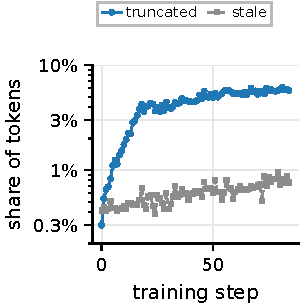
\includegraphics[width=\linewidth]{figures/trigger_a.pdf}\\[-2pt]{\small (a)}
\end{minipage}\hfill
\begin{minipage}[t]{0.325\linewidth}\centering
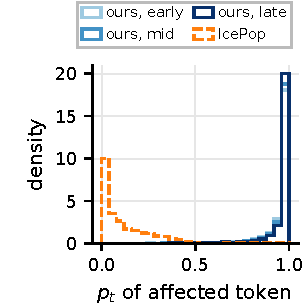
\includegraphics[width=\linewidth]{figures/trigger_b.pdf}\\[-2pt]{\small (b)}
\end{minipage}\hfill
\begin{minipage}[t]{0.325\linewidth}\centering
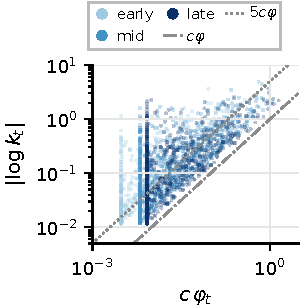
\includegraphics[width=\linewidth]{figures/trigger_c.pdf}\\[-2pt]{\small (c)}
\end{minipage}
\caption{What the band acts on during training (deployed operator, seed one; tokens logged every ten optimizer calls). (a) Fraction of truncated tokens per step (blue) and share of tokens whose rollout version is behind the current one (grey): the trigger rate rises from $0.3\%$ to about $5.5\%$ over the first forty steps and then stays flat, one order of magnitude above the stale share. (b) Training-side confidence $p_t$ of the affected tokens: the truncated tokens of our operator in the early, middle, and late third of training (blue, light to dark) concentrate at $p_t\to1$, whereas the tokens masked by IcePop in its own run (orange, dashed) concentrate at $p_t\to0$; the two operators act on complementary populations. (c) Magnitude $|\log k_t|$ of truncated tokens against the scale-channel width $c\varphi_t$ of their training phase, with $c$ fitted per phase; the dash-dotted and dotted lines mark $c\varphi_t$ and $5c\varphi_t$. Truncated tokens sit at $4$ to $7$ times the local width (median), and the vertical columns at the left are tokens on the floor $\varphi_t=\kappa$.}
\label{fig:trigger}
\end{figure}

Figure~\ref{fig:trigger} shows what the band does over the course of training. The trigger rate rises from $0.3\%$ to about $5.5\%$ during the first forty steps and then plateaus, one order of magnitude above the share of version-stale tokens, which stays between $0.4\%$ and $0.9\%$. Between $87\%$ and $90\%$ of the truncated tokens have $1-p_t<0.1$, and their median $|\log k_t|$ is $0.09$ to $0.10$ in every phase, which is $4$ to $7$ times the scale-channel width of that phase. In standardized training-time units, $49\%$ of the truncated tokens exceed $\zeta=5$ at $\lambda_+=2.3$ and $93\%$ do at $\lambda_+=6.7$, and among the truncated tokens the share of version-stale tokens is $3.0\%$, five times its base rate. Panel (b) is the clearest statement of the difference between the two operators: IcePop removes low-confidence tokens whose ratio leaves a fixed interval, and the band truncates high-confidence tokens whose displacement is large relative to their local width; the acceptance regions of all four operators are drawn in Figure~\ref{fig:regions} of the appendix. Panels (a) and (c) also record a fact about the training run itself: the scale constant grows from $0.61$ to $1.67$ between the first and last third of training while the width at high confidence stays small, so a slope calibrated on the base model becomes tighter in standardized units as training proceeds. This is the mechanism behind the FP8 result and the reason that the compilation $\lambda_+=c\tau^\star$ should be applied to the serving configuration at hand.
